\documentclass[tikz,border=2pt]{standalone}
\renewcommand{\familydefault}{\sfdefault}
\usetikzlibrary{arrows.meta,calc,positioning}
\tikzset{every picture/.style={line width=1pt, >=Stealth},
         hl/.style={fill=black, fill opacity=0.12, text opacity=1}}
\begin{document}
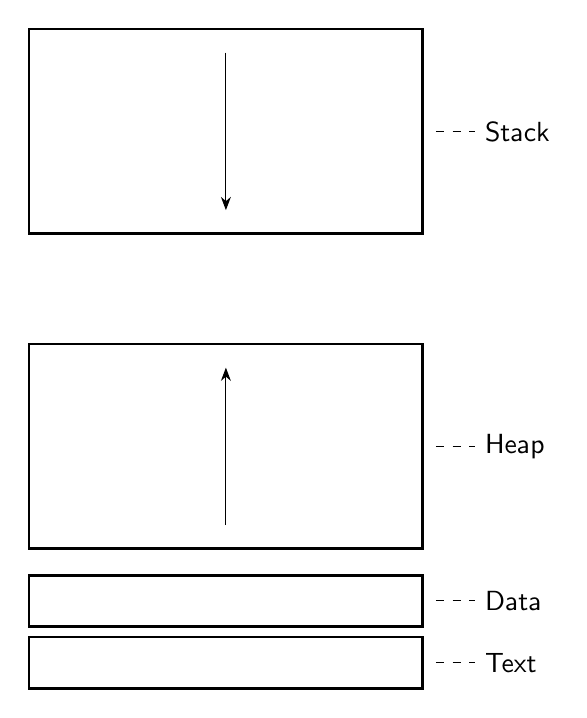
\begin{tikzpicture}[region/.style={draw, minimum width=5cm}]
  % High addresses at the top; the stack grows down and the heap grows up.
  \node[region, minimum height=2.6cm] (stack) at (0, 0) {};
  \draw[->, thin] (0, 1) -- (0, -1);
  \node[region, minimum height=2.6cm] (heap) at (0, -4) {};
  \draw[->, thin] (0, -5) -- (0, -3);
  \node[region, minimum height=0.65cm, below=0.3cm of heap] (data) {};
  \node[region, minimum height=0.65cm, below=0.1cm of data] (text) {};
  \foreach \r/\name in {stack/Stack, heap/Heap, data/Data, text/Text}
    \draw[thin, dashed] ([xshift=0.15cm]\r.east) -- ++(0.5, 0) node[right] {\name};
\end{tikzpicture}
\end{document}
